\documentclass[12pt,a4paper]{report}

\usepackage[utf8]{inputenc}
\usepackage[spanish]{babel}
\usepackage{graphicx}
\usepackage{amsmath}
\usepackage{amssymb}
\usepackage{hyperref}
\usepackage{comment}
\usepackage{geometry}
\usepackage{caption}
\usepackage{subcaption}
\geometry{a4paper, margin=1in}

\title{Segmentación Multimodal para detección de Animales en Entornos Naturales}
\author{
    Jorge Urbón Burgos \\
    \texttt{777295@unizar.es}
    \and
    Supervisor: Rosario Aragües \\
    \texttt{raragues@unizar.es}
    \and
    Co-Supervisor: Jesús Bermúdez \\
    \texttt{bermudez@unizar.es}
}
\date{\today}

\begin{document}

\maketitle

\begin{abstract}
% TODO: add abstract
\end{abstract}

\tableofcontents

\chapter{Introduction}
\label{chap:introduction}
La segmentación de imágenes es una tarea fundamental en el campo de la visión por computador y ha sido ojeto de investigación en \textit{Deep Learning} debido a su importancia en aplicaciones como la detección y clasificación de objetos. En este trabajo, se proponen diferentes modelos de segmentación multimodal a partir de imágenes infrarojas \texttt{IR} y mapas de profundidad \texttt{D} con el fin de obtener una segmentación y clasificación precisas de animales en un entorno natural. Para ello, se empleará un \textit{dataset} más detallado en la sección \ref{subsec:lindenthal_dataset} y se analizarán diferentes modelos del estado del arte, así como los resultados obtenidos con diferentes técnicas de pre-procesado.
La introducción de técnicas multimodales en la segmentación de imágenes puede suponer una gran mejora en las tareas de pastoreo y vigilancia de animales debido a un incremento en la información disponible, lo que permitiría una mejor segmentación y clasificación de los animales en la escena.

\section{Trabajos Relacionados}
\label{sec:related_work}
A pesar de que la segmentación de imágenes ha sido profundamente estudiada en la última década, suponiendo un gran avance en la implementación de sistemas de detección y clasificación de objetos. Aquí encontramos proyectos tan relevantes como \texttt{YOLO} (\cite{YOLO!!!!!}), \texttt{Mask R-CNN} (\cite{maskrcnn}) o \texttt{DeepLab} (\cite{deeplab}). Sin embargo, la mayoría de estos modelos se han centrado en la segmentación de imágenes \texttt{RGB} o de una única modalidad, siendo que proyectos como \cite{MULTIMODALDEEJEMPLO} han demostrado la utilidad de contar con información de diferentes modalidades para la segmentación de imágenes. Aquí, podemos encontrar modelos como TODO: MODELOS MULTIMODALES DE EJEMPLO.

\section{Objetivos}
\label{sec:objectives}
El objetivo de este trabajo es, por tanto, la verificación de la utilidad de las técnicas multimodales en la segmentación de imágenes de animales en un entorno natural con el fin de demostrar su utilidad en tareas como el pastoreo y la vigilancia de animales. Para ello, se analizarán diferentes modelos del estado del arte y se propondrán diferentes técnicas de pre-procesado.
TODO: METER MAS COSAS Q VAYA HACIENDO Y TAL

\chapter{Metodología}
\label{chap:methodology}
\section{Datos}
\label{sec:data}
\subsection{Lindenthal Camera Traps Dataset}
\label{subsec:lindenthal_dataset}
Dado el objetivo que tiene este trabajo de verificar la utilidad de las técnicas multimodales en la segmentación de imágenes de animales en un entorno natural, se requiere de un \textit{dataset} que contenga parejas de imágenes multimodales sincronizadas y etiquetadas para el entrenamiento del modelo. De entre los \textit{datasets} públicos disponibles, el más completo y adecuado para este propósito se trata de \texttt{Lindenthal Camera Traps} presentado por \cite{haucke2021exploitingdepthinformationwildlife}, por lo que durante este proyecto se empleará una parte\footnote{A pesar de que este \textit{dataset} cuenta con 775 secuencias de video que incluyen información \texttt{RGB} durante el día o \texttt{IR} durante la noche, así como mapas de profundidad en ambos casos, tan solo fueron etiquetados para su uso como \textit{Ground Truth} 12 videos nocturnos, de los cuales se etiqueraría cada décimo fotograma.} del mismo. Este \textit{dataset} está constituido por imágenes de animales en el Zoo de Lindenthal, Colonia, obtenidas con una cámara estéreo \texttt{Intel RealSense D435} y en el que se incluyen imágenes infrarojas (\texttt{IR}) con una profundidad de 8 bits y mapas de profundidad (\texttt{D}) con una profundidad de 16 bits en los que el valor de cada pixel representa la distancia en milimetros\footnote{El sensor \texttt{Intel RealSense D435} cuenta con la capacidad de obtener imágenes estéreo de forma activa empleando ambas cámaras infrarojas mediante la proyección de un patrón infrarojo en la escena, sin embargo al haberse construido este dataset a partir de imagenes nocturnas en las que dicho patrón sería visible al sensor \texttt{IR}, se optó por generar los mapas de profundidad \texttt{D} mediante el uso de la cámara estéreo en modo pasivo.}. Ambas modalidades se encuentran ya alineadas y sincronizadas, lo que permite un fácil acceso a la información de ambas modalidades. Además, el etiquetado de los animales se encuentra en formato \texttt{COCO}. En la figura \ref{fig:base-data-lindenthal} se muestra un ejemplo de una pareja de imágenes \texttt{IR} y \texttt{D} del \textit{dataset}. La captura de estas imagenes se realiza desde el tejado de un establo, lo que permite una vista elevada de los animales en la escena. Además, los datos se capturan exclusivamente cuando se da algun tipo de movimiento, por lo que en el \textit{setup} indicado se incluye un sensor infrarojo pasivo (\texttt{PIR}) que actúa como sensor de movimiento.
\begin{figure}
    \centering
    \begin{subfigure}{0.45\textwidth}
        \centering
        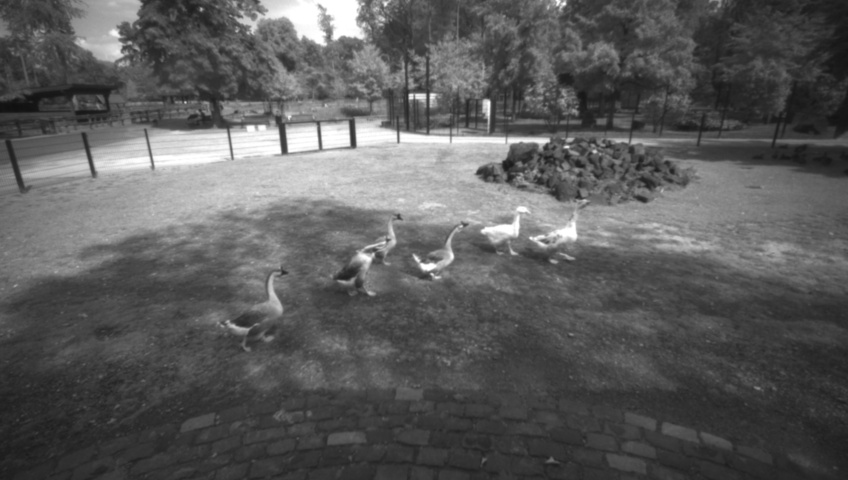
\includegraphics[width=\textwidth]{media/data/ir_gueese.jpg}
        \caption{Imagen \texttt{IR}}
    \end{subfigure}
    \hfill
    \begin{subfigure}{0.45\textwidth}
        \centering
        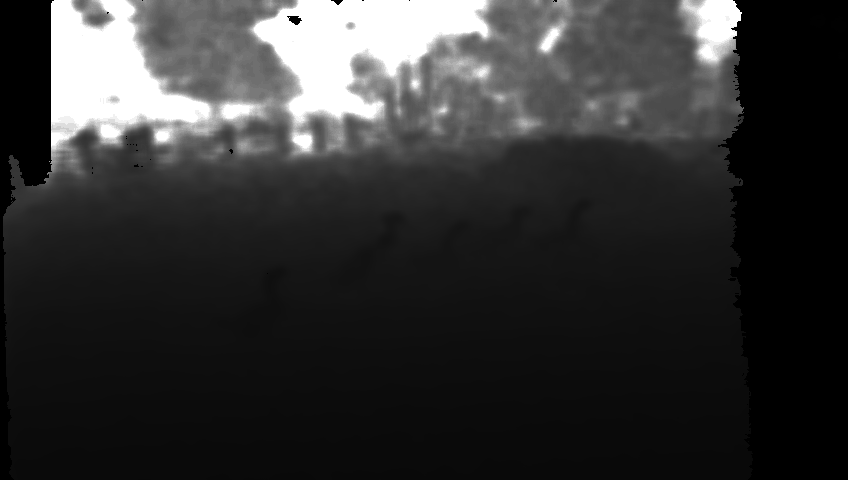
\includegraphics[width=\textwidth]{media/data/depth_gueese.png}
        \caption{Imagen de profundidad}
    \end{subfigure}
    \caption{Ejemplo de una pareja \texttt{IR}-\texttt{D} del \textit{dataset} \texttt{Lindenthal Camera Traps}}
    \label{fig:base-data-lindenthal}
\end{figure}

\subsubsection{Desglose del \textit{Dataset}}
El \textit{dataset} consiste en doce videos para los que se ha etiquetado cada décimo fotograma, lo que supone un total de 412 pares \texttt{IR}-\texttt{D} con 1038 instancias etiquetadas en formato \texttt{COCO} que incluyen la máscara, la caja delimitadora de la misma, la categoría y un identificador único para cada uno de los animales. Las categorías de animales presentes en el dataset son \textbf{Deer}, \textbf{Goat}, \textbf{Donkey} y \textbf{Goose}, siendo considerado todo lo demás descartable, es decir, parte de la categoría \textbf{Background}. En la figura \ref{fig:dataset-breakdown} se muestra un desglose de la frecuencia de aparición de cada categoría en el dataset y se puede observar el amplio desbalanceo entre distintas categorías, por lo que cabe esperar que el modelo tenga ciertas dificultades a la hora de segmentar las categorías menos frecuentes como por ejemplo \textbf{Donkey}.
\begin{figure}
    \centering
    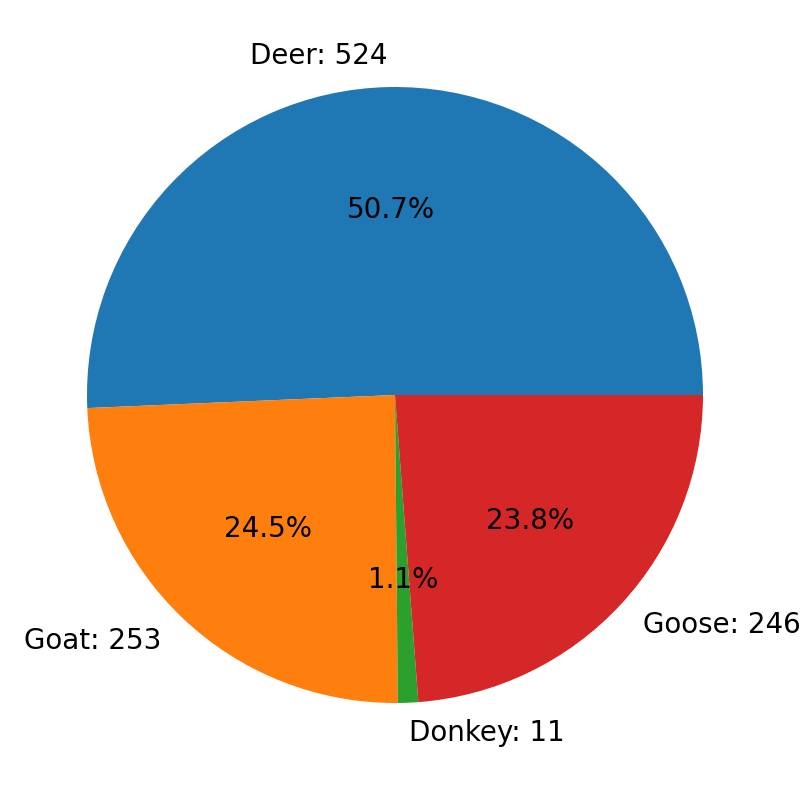
\includegraphics[width=0.5\textwidth]{media/data/dataset_breakdown.png}
    \caption{Desglose de la frecuencia de aparición de cada categoría en el dataset}
    \label{fig:dataset-breakdown}
\end{figure}
Por otra parte, este \textit{dataset} se mezclará aleatoriamente y se dividirá en dos partes: el 85\% de las imágenes se emplearán para entrenamiento y el 15\% restante para validación de los resultados con el fin de aplicar técnicas como el \texttt{EarlyStopping} o simplemente para una verificación manual del buen entrenamiento durante el proceso. En la figura \ref{fig:tagged-example} se muestra un ejemplo de un par \texttt{IR}-\texttt{D} con sus respectivas máscaras de segmentación extraidas del etiquetado \texttt{COCO}.
\begin{figure}
    \centering
    \begin{subfigure}{0.45\textwidth}
        \centering
        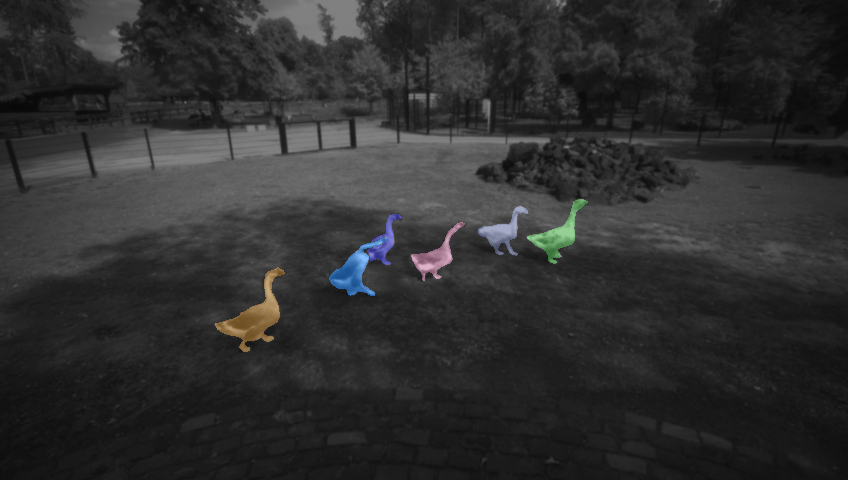
\includegraphics[width=\textwidth]{media/data/mask_gueese_ir.png}
        \caption{Imagen \texttt{IR} etiquetada}
    \end{subfigure}
    \hfill
    \begin{subfigure}{0.45\textwidth}
        \centering
        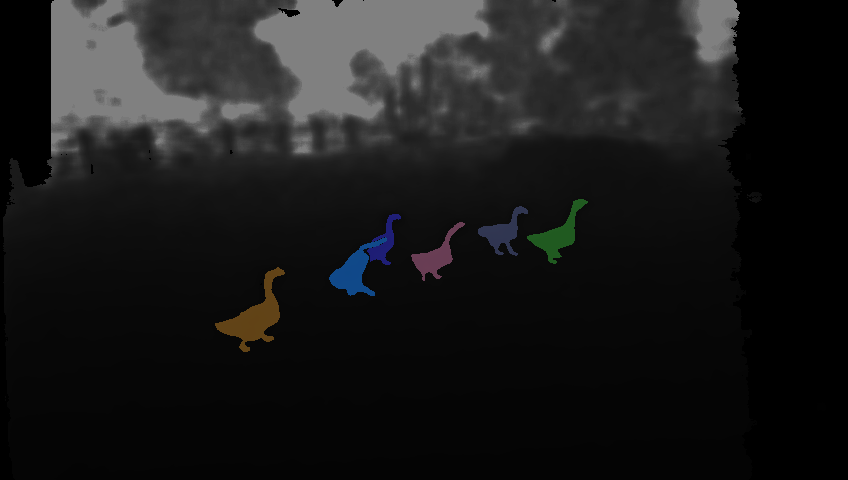
\includegraphics[width=\textwidth]{media/data/mask_gueese_de.png}
        \caption{Imagen \texttt{D} etiquetada}
    \end{subfigure}
    \caption{Ejemplo de una pareja \texttt{IR}-\texttt{D} del \textit{dataset} \texttt{Lindenthal Camera Traps}}
    \label{fig:tagged-example}
\end{figure}

\section{Modelo}
\label{sec:model}
El modelo a implementar, \texttt{CrossModalFusion} (\texttt{CMX}), fue presentado por \cite{zhang2023cmxcrossmodalfusionrgbx} y propone una arquitectura de fusión de características de forma interactiva implementando rectificación de características inter-modal y bidireccional, así como atención cruzada secuencia a secuencia, lo que permite interacciones inter-modales más ricas y efectivas. La arquitectura propuesta por \cite{zhang2023cmxcrossmodalfusionrgbx} se muestra en la figura \ref{fig:cmx-architecture}, y su principal característica se encuentra en la rectificación inter-modal de las características a la salida de cada una de las capas del encoder, así como en la fusión de estas características rectificadas para su uso como características de menor nivel en la entrada al decoder. Además, este modelo incluye un \textit{backbone} con pesos pre-entrenados en \texttt{ImageNet} que permiten un aprendizaje más efectivo de las características de la escena gracias a la gran cantidad de datos de entrenamiento con los que cuenta \texttt{ImageNet}. Sin embargo, dado que la versión de \texttt{ImageNet} empleada es puramente \texttt{RBG}, se requiere de un entrenamiento algo más intensivo para adaptar dichos pesos a las nuevas modalidades de entrada \texttt{IR} y \texttt{D}.
\begin{figure}
    \centering
    \includegraphics[width=\textwidth]{media/model/cmx_architecture.png}
    \caption{Arquitectura propuesta por \cite{zhang2023cmxcrossmodalfusionrgbx}}
    \label{fig:cmx-architecture}
\end{figure}


\subsection{Entrenamiento}
\label{subsec:training}
El entrenamiento del modelo es realizado en un portátil con una tarjeta gráfica \texttt{NVIDIA GeForce GTX 1650} con 4GB de memoria \texttt{VRAM} y un procesador \texttt{Intel Core i5-10300H} con 8 núcleos y 16 hilos, así como 16GB de memoria \texttt{RAM}. Debido a los bajos resursos de los que se dispone, se optará por un entrenamiento en una única GPU y un tamaño de \textit{batch} de 2. Además, como se ha mencionado en el anterior apartado, se empleará un \textit{backbone} pre-entrenado en \texttt{ImageNet} y se aplicará la técnica de \textit{transfer learning} para adaptar el modelo a las características de los datos de entrada. Se empleará la función de pérdida \texttt{CrossEntropyLoss} y el optimizador \texttt{Adam} con una tasa de aprendizaje de $10^{-6}$ dinámica. El modelo se entrenará durante 500 épocas con un tamaño de \textit{batch} de 2. Por último, para fomentar el aprendizaje de las características de forma independiente en ambas modalidades, se realizará un \textit{modality dropout} con una probabilidad de 0.5 decreciente con el número de épocas con el fin de que el modelo aprenda a desenvolverse con una sola modalidad en el caso de que, por el motivo que sea, la otra no esté disponible.

Además, como se precisa en la subsección \ref{subsec:preprocessing_techniques}, se analizarán diferentes técnicas de pre-procesado con el fin de determinar cuál puede aumentar la información disponible para el modelo y, por tanto, mejorar la segmentación de las imágenes.

\section{Técnicas de Pre-Procesado}
\label{subsec:preprocessing_techniques}
Cuando vamos a usar una imagen como input para un modelo de segmentación, se debe tener en cuenta el formato en el que se desea representar la información que se le proporciona al modelo. En este caso, se cuenta con dos modalidades de entrada: \texttt{IR} y \texttt{D}, por lo que se deben considerar las distintas técnicas de preprocesado que se pueden aplicar a cada modalidad para obtener un mejor resultado en la segmentación.

Así como aumentar la información que otorga el canal \texttt{IR} es una tarea complicada, ya que la imagen ya cuenta con una calidad aceptable, el canal \texttt{D} es el que más ruido presenta y, quizá, el que el modelo tenga más dificultades de entender debido a su escasa similaridad con los datos de pre-entrenamiento en \texttt{ImageNet}. Por tanto, se propone aplicar las técnicas de pre-procesado exclusivamente al canal \texttt{D} con el fin de aumentar la información disponible para el modelo e, idealmente, que este aprenda a emplearlos con el fin de mejorar la segmentación de las imágenes.

Existe una variedad de técnicas de pre-procesado que aprovechan los tres canales de entrada del modelo para así lograr un \textit{input} capaz de aportar mayor cantidad de información al modelo de segmentación. A continuación, se presentan las técnicas de pre-procesado que se proponen para este trabajo.

\begin{figure}
    \centering
    \begin{subfigure}{0.45\textwidth}
        \centering
        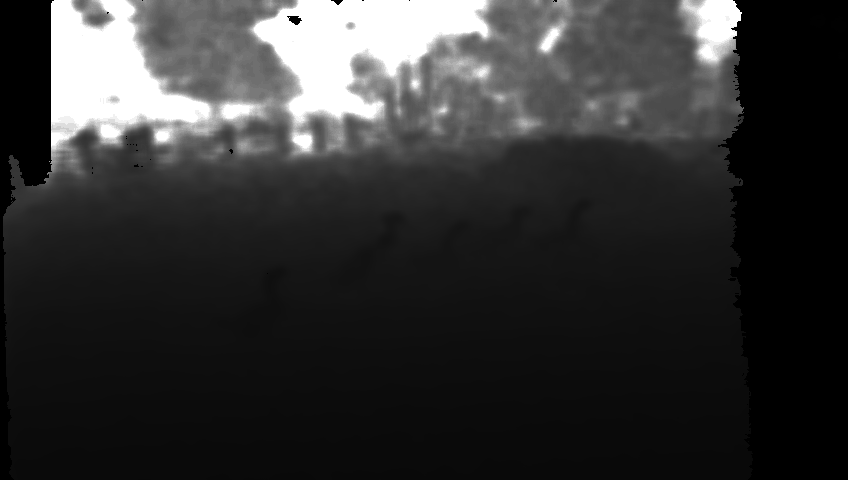
\includegraphics[width=\textwidth]{media/data/depth_gueese.png}
        \caption{Imagen de profundidad base}
        \label{fig:depth-base}
    \end{subfigure}
    \hfill
    \begin{subfigure}{0.45\textwidth}
        \centering
        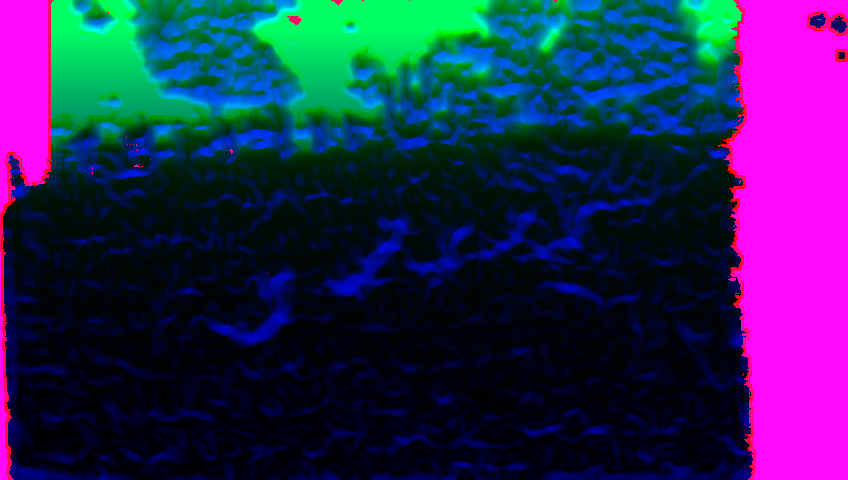
\includegraphics[width=\textwidth]{media/data/hha_gueese.png}
        \caption{Profundidad colorizada con HHA}
        \label{fig:hha-colorization}
    \end{subfigure}
    \vfill
    \begin{subfigure}{0.45\textwidth}
        \centering
        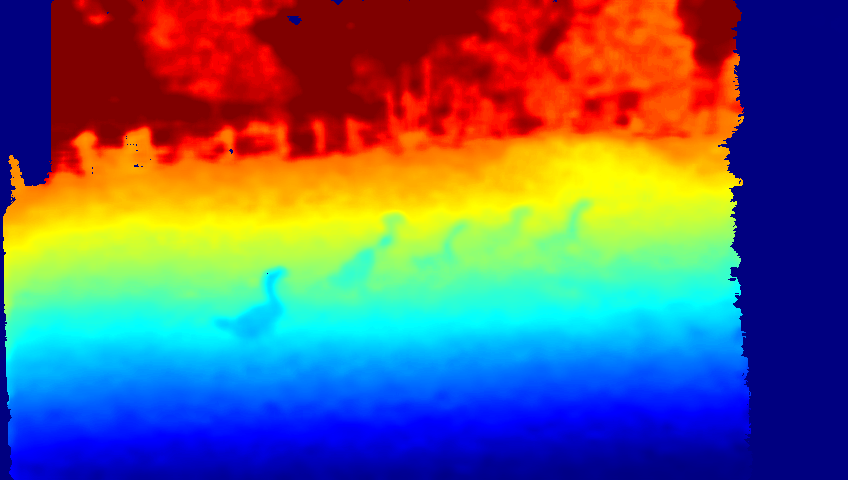
\includegraphics[width=\textwidth]{media/data/jet_gueese.png}
        \caption{Profundidad colorizada con \textit{Jet}}
        \label{fig:jet-colorization}
    \end{subfigure}
    \hfill
    \begin{subfigure}{0.45\textwidth}
        \centering
        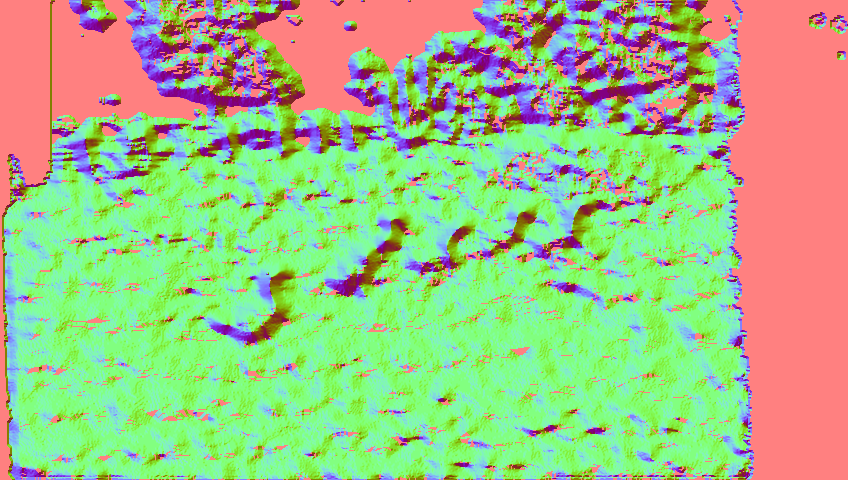
\includegraphics[width=\textwidth]{media/data/normal_gueese.png}
        \caption{Normales en la imagen de profundidad}
        \label{fig:normals-colorization}
    \end{subfigure}
    \caption{Comparación entre las distintas técnicas de post-procesado}
    \label{fig:preprocessing-comparison}
\end{figure}
\begin{comment}
    '20200807061001/color/000051.jpg'
\end{comment}

\begin{comment}
\subsubsection{Equalización del Histograma}
La primera técnica de postprocesado a implementar consiste en la equalización del histograma de valores en la imagen. Esto puede suponer una gran mejora en la forma en la que se representan las imágenes debido a que no todo el rango de valores de intensidad es aprovechado dado a que la mayoría de los objetos de interés se encuentran a una distancia relativamente baja de la cámara. Equalizar el histograma puede permitir destacar ciertos objetos que de otra forma no serían tan visibles.
\begin{figure}
    \centering
    \begin{subfigure}{0.45\textwidth}
        \centering
        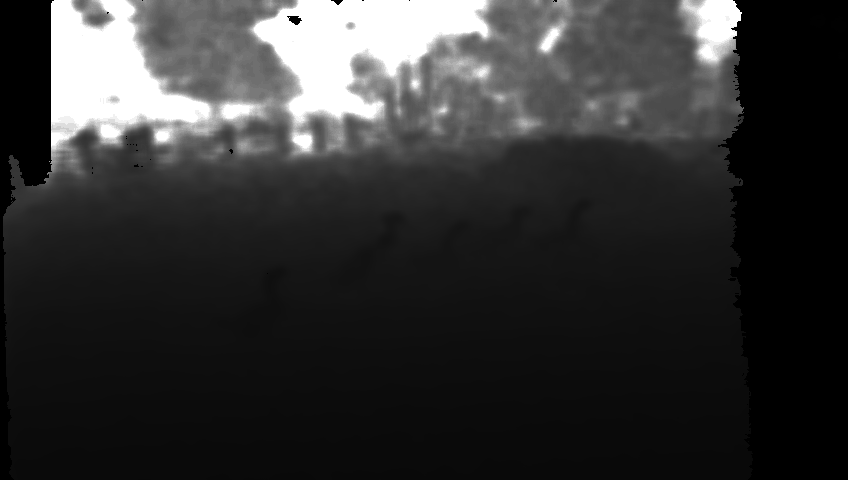
\includegraphics[width=\textwidth]{media/data/depth_gueese.png}
        \caption{Imagen de profundidad base}
    \end{subfigure}
    \hfill
    \begin{subfigure}{0.45\textwidth}
        \centering
        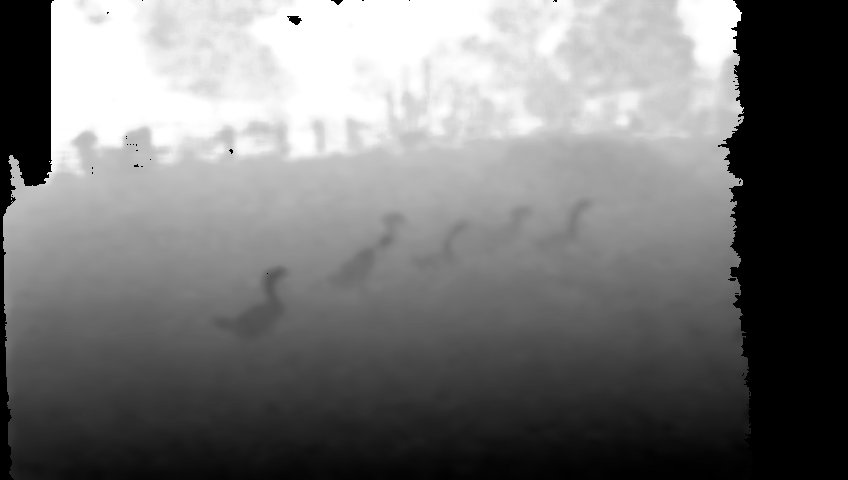
\includegraphics[width=\textwidth]{media/data/deptheq_gueese.png}
        \caption{Histograma equalizado}
    \end{subfigure}
    \caption{Comparación entre la imagen de profundidad base y la imagen con el histograma equalizado}
    \label{fig:depth-histeq-comparison}
\end{figure}
Como se puede observar en la figura \ref{fig:histogram-comparison}, la ecualización del histograma permite un mayor reparto de los valores de intensidad en la imagen, lo que aprovecha aquellos rangos menos utilizados en la imagen original permitiendo así un mayor contraste entre los rangos más utilizados en la imagen original como se puede observar en la figura \ref{fig:depth-histeq-comparison}.
Esta técnica, sin embargo, puede no ser adecuada para otras aplicaciones, ya que se pierde la información real sobre la distancia de los objetos a la cámara.
\begin{figure}
    \centering
    \begin{subfigure}{0.45\textwidth}
        \centering
        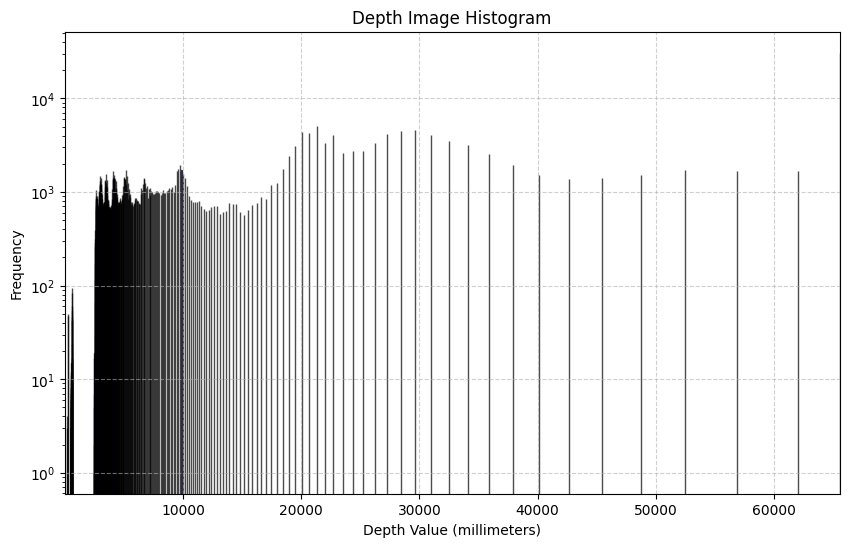
\includegraphics[width=\textwidth]{media/data/normal_histogram.png}
        \caption{Histograma de la imagen de profundidad base}
    \end{subfigure}
    \hfill
    \begin{subfigure}{0.45\textwidth}
        \centering
        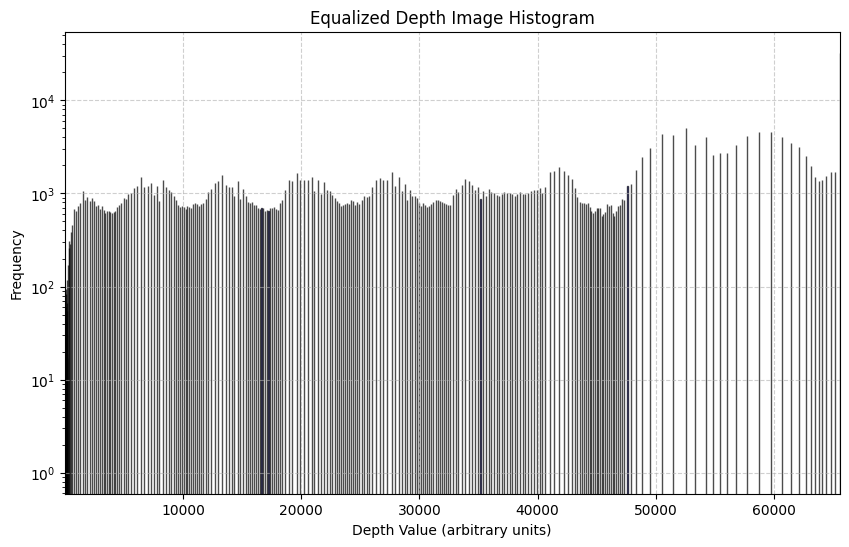
\includegraphics[width=\textwidth]{media/data/equalized_histogram.png}
        \caption{Histograma de la imagen con el histograma equalizado}
    \end{subfigure}
    \caption{Comparación entre los histogramas de la imagen de profundidad base y la imagen con el histograma equalizado}
    \label{fig:histogram-comparison}
\end{figure}
\end{comment}

\subsection{HHA Encoding}
\label{subsubsec:hha_encoding}
Esta técnica, propuesta por \cite{gupta2014learningrichfeaturesrgbd} usa los tres canales de la imagen de entrada para codificar las siguientes tres características:
\begin{itemize}
    \item Altura sobre el suelo
    \item Disparidad horizontal
    \item Ángulo con respecto a la gravedad
\end{itemize}
Estas colorización, además de implementar características que difícilmente serían aprendidas por el modelo si no se codificaran en la imagen de entrada, aprovecha los tres canales de entrada al \textit{encoder}, por lo que los pesos ya preentrenados en \textit{ImageNet} pueden ser empleados para una mejor comprensión de la escena. A pesar de que esta colorización permite calcular las características mencionadas, el tiempo de cómputo necesario para realizar esta operación puede ser elevado, por lo que la aplicación de esta técnica podría limitar los casos de uso en los que se emplee. Un ejemplo de esta técnica se muestra en la figura \ref{fig:hha-colorization}.

\subsection{Colorizacón Jet}
\label{subsubsec:jet_colorization}
Como se propone en \cite{eitel2015multimodaldeeplearningrobust}, otra posible técnica es la colorización de la imagen de entrada usando el esquema de color \textit{Jet} como se puede ver en la figura \ref{fig:jet-colorization}, lo que implica la asignación de un valor \textit{RGB} a cada píxel dependiendo de su valor de intensidad. Esto, al contrario de lo que sucede en \ref{subsubsec:hha_encoding}, no amplía la información disponible para el modelo de ninguna forma, ya que en la imagen de entrada se sigue representando la distancia de los objetos a la cámara, pero podría resultar en mayor facilidad de aprendizaje para el modelo debido al uso de los pesos pre-entrenados en \texttt{ImageNet} y el mayor contraste entre los objetos en la escena. Este proceso, como se menciona en \cite{eitel2015multimodaldeeplearningrobust}, puede ser más rápido que el de HHA, pero no necesariamente más efectivo.

\subsection{Colorización por Distancia}
Considerando los resultados obtenidos por Jet, se propone en una técnica de colorización que, si bien puede no resultar tan visualmente atractiva para el ojo humano como su alternativa, podría codificar la distancia de forma más efectiva para el modelo al establecer una relación lineal entre los valores de profundidad y el valor de los canales de la imagen final. De tal forma, esta técnica también se basa en asignar un valor \texttt{RGB} a cada píxel dependiendo de su valor de intensidad, pero en este caso se determinará que los objetos más lejanos serán más dominados por el canal \texttt{R}, mientras que los objetos más cercanos serán más dominados por el canal \texttt{B} pasando por el canal \texttt{G} en el rango intermedio. La interpolación de los valores de distancia a estos valores podría ser aprendida por el modelo de forma algo más efectiva que en el caso de Jet a pesar de su menor contraste al ojo humano.

\subsection{Normales}
\label{subsubsec:normals}
Siguiendo lo propuesto por \cite{eitel2015multimodaldeeplearningrobust}, una mejor y más rápida solución de postprocesado consiste en la codificación de las normales en la imagen de entrada. Esta técnica consiste en calcular el vector normal de la superficie de cada pixel partiendo de la imagen de profundidad y codificarlo en los tres canales del \textit{input} del modelo. Esto permite al modelo aprender características de la escena que de otra forma serían difíciles de aprender, como la orientación de los objetos en la escena. La imagen final, mostrada en la figura \ref{fig:normals-colorization}, se obtiene calculando las derivadas parciales respecto a $x$ e $y$ de los valores de profundidad en la imagen y normalizando el vector resultante como se muestra en la ecuación \ref{eq:normals}.

\begin{equation}
    \begin{aligned}
        \hat{n} = \frac{(n_x, n_y, 1)}{\sqrt{n_x^2 + n_y^2 + 1}} \\
        n_x = \frac{\partial z}{\partial x}, n_y = \frac{\partial z}{\partial y} 
    \end{aligned}
    \label{eq:normals}
\end{equation}

\subsection{Comparación de Técnicas}
\label{subsubsec:techniques_comparison}
Las distintas técnicas anteriores presentan diferentes resultados tras su evaluación, tal y como se puede ver en las matrices de confusión presentes en el anexo (TODO: referir al anexo!!!), en la tabla \ref{tab:techniques_comparison} se muestra la media de la precisión \texttt{IoU} obtenida por cada una de las técnicas de pre-procesado propuestas, donde se puede apreciar que la colorización \texttt{Jet} es la mejor opción cuando ambas modalidades están disponibles, mientras que no emplear ninguna técnica de pre-procesado es la mejor opción cuando solo se cuenta con la imagen \texttt{D} o \texttt{IR}. Esto se debe posiblemente a que TODO: expliar esta movida!!!

Además, como se puede ver en las matrices de confusión que se encuentran en el anexo (TODO: referir al anexo!!!) todas estas técnicas comparten una precisión extremadamente alta al diferenciar entre clases, siendo la confusión con el fondo la principal fuente de error en la segmentación de las imágenes. Un ejemplo del resultado de la segmentación de una imagen empleando colorización \texttt{Jet} se muestra en la figura \ref{fig:segmentation-example}.

\begin{table}[!h]
    \centering
    \begin{tabular}{|c|c|c|c|}
        \hline
        \textbf{Técnica} & \textbf{IR+D} & \textbf{Depth} & \textbf{InfraRed} \\
        \hline
        Sin Pre-Procesado & 90.54\% & \textbf{74.56\%} & \textbf{90.51}\% \\
        HHA Encoding & 90.60\% &  41.83\% &  89.78\%\\
        Colorización Jet & \textbf{90.78\%} & 73.54\% & 90.23\%\\
        Colorización por Distancia & 89.92\% & 73.58\% & 88.70\%\\
        Normales & 90.76\% & 72.49\% & 88.22\%\\
        \hline
    \end{tabular}
    \caption{Comparación de las técnicas de pre-procesado propuestas}
    \label{tab:techniques_comparison}
\end{table}

\chapter{Results}
\label{chap:results}
% TODO: add results

\bibliography{refs.bib}
\bibliographystyle{IEEEtran}

\appendix
\label{app:appendix_a}
% TODO: whatever appendices :)

\end{document}